\subsection{Simulazione degli eventi tramite metodo Monte Carlo}

Per avere una migliore stima della frazione accettata di eventi a 3 fotoni si è ricorsi ad una simulazione Monte Carlo. Si è perciò simulato un numero molto grande di eventi ($10^{10}$) e si è contato quanti di questi hanno interagito con tutti e tre i rivelatori, considerati dei dischi con efficienza 100\%.\\

Per ogni evento sono stati simulati separamente la $\varphi$ del primo fotone, la $\theta$ del primo fotone, i due angoli tra i fotoni all'interno del piano, e la direzione del piano su cui giace il decadimento (che ruota intorno alle direzione del primo fotone).\\

Dato che vogliamo che il primo fotone sia isotropo, è necessario che 
\begin{equation}
	\frac{\dd p}{\dd\Omega} = \frac{\dd^2 p}{\dd\theta \dd\varphi \sin(\theta)} = \mathrm{const} \rightarrow \frac{\dd^2 p}{\dd\theta \dd\varphi} \propto \sin(\theta)
\end{equation}
quindi, dato che le probabilità di $\varphi$ e $\theta$ sono indipendenti
\begin{align}
	\frac{\dd p}{\dd\varphi}& = \frac{1}{2\pi} \label{eq:varphi}\\
	\frac{\dd p}{\dd\varphi}& = \frac{\sin(\theta)}{2} \label{eq:theta}
\end{align}
distribuzioni facilmente campionabili tramite il metodo della trasformata inversa.\\

Per la simulazione degli angoli tra i due fotoni si è applicato \textit{rejection method} alla funzione
\begin{equation}
	\frac{\dd^3 p}{\dd\alpha_1 \dd\alpha_2 \dd\alpha_3} = \frac{\left(\sum_{i=1}^{3} \left(1-\cos(\alpha_i)\right)^2\right)\cdot\left(\prod_{i=1}^{3} \sin(\alpha_i)\right)}{\sum_{i=1}^{3} \sin(\alpha_i)}
\end{equation}
dove $\alpha_3=2\pi-\alpha_1-\alpha_2$.\\

La direzione del piano è più delicata da generare. Per generare eventi sensati si vorrebbe infatti che tale direzione sia isotropa. Chiamate $\theta_p$ e $\varphi_p$ le coordinate sferiche della perpendicolare al piano, si ha che devono soddisfare le equazioni \ref{eq:varphi} e \ref{eq:theta}. L'equazione in $\varphi_p$ è banalmente soddisfatta causa dell'isotropia della $\varphi$ del primo fotone, mentre la $\theta_p$ è più delicata.
L'espressione di $\theta_p$ in funzione di $\theta$ direzione del primo fotone e $\alpha$ angolo di rotazione del piano è
\begin{equation}
	\cos(\theta_p)=\cos(\alpha)\cdot\sin(\theta)
\end{equation}
si ha che la funzione di ripartizione di $\cos(\theta_p)$ è
\begin{equation}
\begin{split}
	F(\cos(\bar\theta_p))& = P(\cos(\theta_p) < \cos(\bar\theta_p)) \\
	& = 2\,\int _{\arcsin \left( \cos(\bar\theta_p) \right) }^{1/2\,\pi }\!\int _{0}^{\pi -\arccos \left( {\frac {\cos(\bar\theta_p)}{\sin \left( \theta \right) }} \right) }\!{\it f} \left( \alpha,\theta \right) \sin \left( \theta \right) {d\alpha}\,{d\theta}\\
	&\quad+2\,\int _{0}^{\arcsin \left( \cos(\bar\theta_p) \right) }\!\int _{0}^{\pi }\!{\it f} \left( \alpha,\theta \right) \sin \left( \theta \right) {d\alpha}\,{d\theta}
\end{split}
\end{equation}
dove $f(\alpha\,|\,\theta)$ è la densità di probabilità di $\alpha$ dato $\theta$, la nostra incognita.\\
La densità di probabilità di $\cos(\theta_p)$ è perciò
\begin{equation}
	\frac{\dd F(\cos(\theta_p))}{\dd\cos(\theta_p)} = 2\,\int _{\arcsin \left( \cos(\theta_p) \right) }^{1/2\,\pi }\!f \left( \pi -\arccos \left( {\frac {\cos(\theta_p)}{\sin \left( \theta \right) }} \right) ,\theta \right) {\frac {1}{\sqrt {1-{\frac {{\cos(\theta_p)}^{2}}{ \left( \sin \left( t \right)  \right) ^{2}}}}}}{d\theta}
\end{equation}

Sì è preferito ricavare la densità di $\cos(\theta_p)$ per semplificare i conti, dato che se $\theta_p$ ha densità pari a $\sin(\theta_p)$, $\cos(\theta_p)$ ha una distribuzione uniforme tra -1 e 1.\\
Richiedendo tale condizione si ottiene per $f(\alpha\,|\,\theta)$ l'espressione
\begin{equation}
	f(\alpha\,|\,\theta) = {\frac { \left| \sin \left( \theta \right) \sin \left( \alpha \right) 
 \right| }{ \left[ \pi +2\,\arcsin \left( \cos \left( \alpha \right) 
\sin \left( \theta \right)  \right)  \right] \sin \left( \theta
 \right) }}
\end{equation}
che simuliamo sempre tramite \textit{rejection method}.\\
Come si può vedere dalla Figura \ref{fig:isotrophy}, tale distribuzione risulta in una direzione del piano effettivamente isotropa.\\
\begin{figure}[h]\centering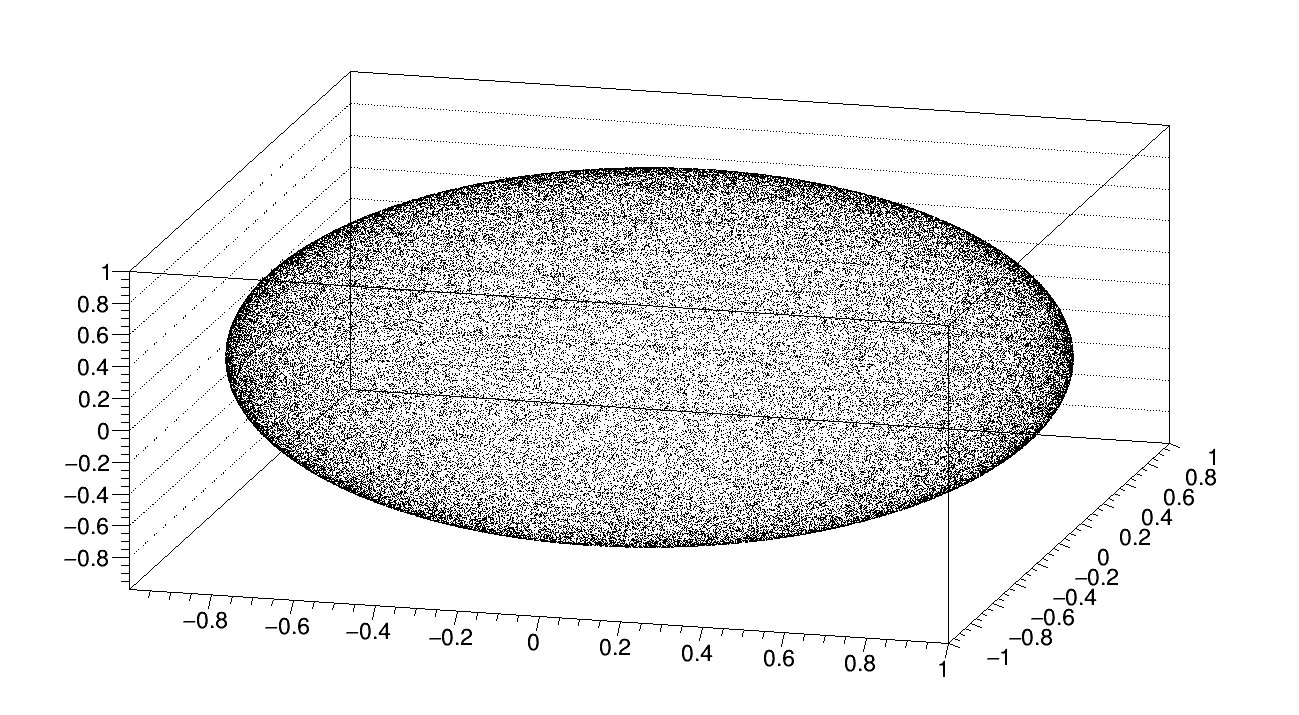
\includegraphics[width=0.9\textwidth]{../../img/isotrophy.png}\caption{Distribuzione delle direzioni della perpendicolare al piano di decadimento. Come si può vedere, la distribuzione è effettivamente isotropa.}\label{fig:isotrophy}\end{figure}


Simulando $1\times 10^{10}$ eventi di questo tipo considerando tre rivelatori a 120$^\circ$ l'uno dall'altro, si ottiene una frazione di eventi accettati di 
$$\nu=0.06580\pm0.00008$$


